% GNUPLOT: LaTeX picture with Postscript
\begingroup
  \makeatletter
  \providecommand\color[2][]{%
    \GenericError{(gnuplot) \space\space\space\@spaces}{%
      Package color not loaded in conjunction with
      terminal option `colourtext'%
    }{See the gnuplot documentation for explanation.%
    }{Either use 'blacktext' in gnuplot or load the package
      color.sty in LaTeX.}%
    \renewcommand\color[2][]{}%
  }%
  \providecommand\includegraphics[2][]{%
    \GenericError{(gnuplot) \space\space\space\@spaces}{%
      Package graphicx or graphics not loaded%
    }{See the gnuplot documentation for explanation.%
    }{The gnuplot epslatex terminal needs graphicx.sty or graphics.sty.}%
    \renewcommand\includegraphics[2][]{}%
  }%
  \providecommand\rotatebox[2]{#2}%
  \@ifundefined{ifGPcolor}{%
    \newif\ifGPcolor
    \GPcolortrue
  }{}%
  \@ifundefined{ifGPblacktext}{%
    \newif\ifGPblacktext
    \GPblacktextfalse
  }{}%
  % define a \g@addto@macro without @ in the name:
  \let\gplgaddtomacro\g@addto@macro
  % define empty templates for all commands taking text:
  \gdef\gplbacktext{}%
  \gdef\gplfronttext{}%
  \makeatother
  \ifGPblacktext
    % no textcolor at all
    \def\colorrgb#1{}%
    \def\colorgray#1{}%
  \else
    % gray or color?
    \ifGPcolor
      \def\colorrgb#1{\color[rgb]{#1}}%
      \def\colorgray#1{\color[gray]{#1}}%
      \expandafter\def\csname LTw\endcsname{\color{white}}%
      \expandafter\def\csname LTb\endcsname{\color{black}}%
      \expandafter\def\csname LTa\endcsname{\color{black}}%
      \expandafter\def\csname LT0\endcsname{\color[rgb]{1,0,0}}%
      \expandafter\def\csname LT1\endcsname{\color[rgb]{0,1,0}}%
      \expandafter\def\csname LT2\endcsname{\color[rgb]{0,0,1}}%
      \expandafter\def\csname LT3\endcsname{\color[rgb]{1,0,1}}%
      \expandafter\def\csname LT4\endcsname{\color[rgb]{0,1,1}}%
      \expandafter\def\csname LT5\endcsname{\color[rgb]{1,1,0}}%
      \expandafter\def\csname LT6\endcsname{\color[rgb]{0,0,0}}%
      \expandafter\def\csname LT7\endcsname{\color[rgb]{1,0.3,0}}%
      \expandafter\def\csname LT8\endcsname{\color[rgb]{0.5,0.5,0.5}}%
    \else
      % gray
      \def\colorrgb#1{\color{black}}%
      \def\colorgray#1{\color[gray]{#1}}%
      \expandafter\def\csname LTw\endcsname{\color{white}}%
      \expandafter\def\csname LTb\endcsname{\color{black}}%
      \expandafter\def\csname LTa\endcsname{\color{black}}%
      \expandafter\def\csname LT0\endcsname{\color{black}}%
      \expandafter\def\csname LT1\endcsname{\color{black}}%
      \expandafter\def\csname LT2\endcsname{\color{black}}%
      \expandafter\def\csname LT3\endcsname{\color{black}}%
      \expandafter\def\csname LT4\endcsname{\color{black}}%
      \expandafter\def\csname LT5\endcsname{\color{black}}%
      \expandafter\def\csname LT6\endcsname{\color{black}}%
      \expandafter\def\csname LT7\endcsname{\color{black}}%
      \expandafter\def\csname LT8\endcsname{\color{black}}%
    \fi
  \fi
    \setlength{\unitlength}{0.0500bp}%
    \ifx\gptboxheight\undefined%
      \newlength{\gptboxheight}%
      \newlength{\gptboxwidth}%
      \newsavebox{\gptboxtext}%
    \fi%
    \setlength{\fboxrule}{0.5pt}%
    \setlength{\fboxsep}{1pt}%
\begin{picture}(5040.00,3772.00)%
    \gplgaddtomacro\gplbacktext{%
      \csname LTb\endcsname%
      \put(396,594){\makebox(0,0)[r]{\strut{}\footnotesize{$0$}}}%
      \csname LTb\endcsname%
      \put(396,954){\makebox(0,0)[r]{\strut{}\footnotesize{$10$}}}%
      \csname LTb\endcsname%
      \put(396,1313){\makebox(0,0)[r]{\strut{}\footnotesize{$20$}}}%
      \csname LTb\endcsname%
      \put(396,1673){\makebox(0,0)[r]{\strut{}\footnotesize{$30$}}}%
      \csname LTb\endcsname%
      \put(396,2032){\makebox(0,0)[r]{\strut{}\footnotesize{$40$}}}%
      \csname LTb\endcsname%
      \put(396,2392){\makebox(0,0)[r]{\strut{}\footnotesize{$50$}}}%
      \csname LTb\endcsname%
      \put(396,2751){\makebox(0,0)[r]{\strut{}\footnotesize{$60$}}}%
      \csname LTb\endcsname%
      \put(396,3111){\makebox(0,0)[r]{\strut{}\footnotesize{$70$}}}%
      \csname LTb\endcsname%
      \put(528,374){\makebox(0,0){\strut{}\footnotesize{$-60$}}}%
      \csname LTb\endcsname%
      \put(1192,374){\makebox(0,0){\strut{}\footnotesize{$-50$}}}%
      \csname LTb\endcsname%
      \put(1856,374){\makebox(0,0){\strut{}\footnotesize{$-40$}}}%
      \csname LTb\endcsname%
      \put(2520,374){\makebox(0,0){\strut{}\footnotesize{$-30$}}}%
      \csname LTb\endcsname%
      \put(3183,374){\makebox(0,0){\strut{}\footnotesize{$-20$}}}%
      \csname LTb\endcsname%
      \put(3847,374){\makebox(0,0){\strut{}\footnotesize{$-10$}}}%
      \csname LTb\endcsname%
      \put(4511,374){\makebox(0,0){\strut{}\footnotesize{$0$}}}%
    }%
    \gplgaddtomacro\gplfronttext{%
      \csname LTb\endcsname%
      \put(88,1852){\rotatebox{-270}{\makebox(0,0){\strut{}\footnotesize{SNR [dB]}}}}%
      \put(2519,154){\makebox(0,0){\strut{}\footnotesize{input [dB]}}}%
      \put(2519,3441){\makebox(0,0){\strut{}\shortstack{16-bit Fixed point \\Cosine $f=0.1$ Q1.15}}}%
      \csname LTb\endcsname%
      \put(1188,1196){\makebox(0,0)[r]{\strut{}\tiny{FFT64}}}%
      \csname LTb\endcsname%
      \put(1188,1042){\makebox(0,0)[r]{\strut{}\tiny{FFT256}}}%
      \csname LTb\endcsname%
      \put(1188,888){\makebox(0,0)[r]{\strut{}\tiny{FFT1024}}}%
      \csname LTb\endcsname%
      \put(1188,734){\makebox(0,0)[r]{\strut{}\tiny{FFT4096}}}%
    }%
    \gplbacktext
    \put(0,0){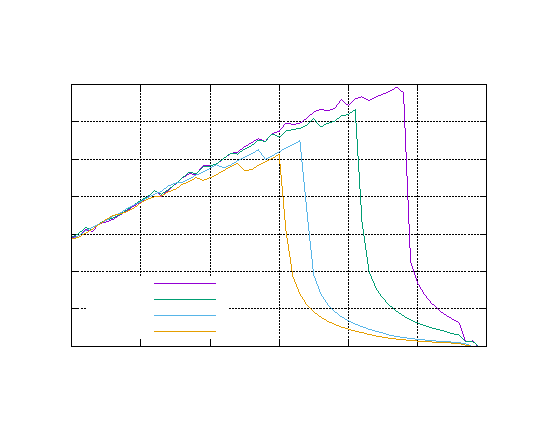
\includegraphics{cosine_DR}}%
    \gplfronttext
  \end{picture}%
\endgroup
